\section{定理}

\begin{figure}[t]
    \centering
    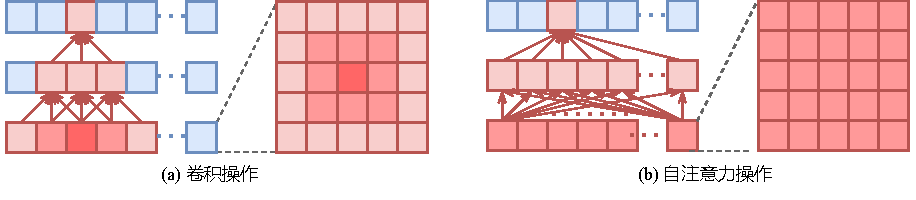
\includegraphics[width=\textwidth]{pics/conv vs attention.pdf}
    \caption{卷积操作和自注意力操作}
    \label{fig:conv_vs_attention}
\end{figure}

卷积神经网络(CNN)和Vision Transformer(ViT)是两种截然不同的模型,前者的主要操作是卷积,而后者的主要操作是自注意力机制。本章节将通过理论推导进行分析,比较CNN和ViT的差异和可能的内在原因。

CNN是一种特殊的神经网络,经典的CNN模型包括AlexNet、VGG、ResNet等,这些模型采用卷积、池化、Batch Normalization、激活函数等操作,通过堆叠这些操作,逐渐提取出输入数据的高层次特征。其中,卷积操作是CNN的核心操作,卷积操作的本质是一种特殊的线性变换,它通过卷积核与输入数据的点乘操作,将输入数据的局部特征提取出来。卷积操作的局部性质使得CNN能够有效地提取空间特征,因此CNN在图像处理领域取得了巨大的成功。卷积操作可以表示为公式\ref{eq:conv}:

\begin{equation}
    \label{eq:conv}
    y_{i, j} = \sum_{m=0}^{k-1} \sum_{n=0}^{k-1} x_{i+m, j+n} \cdot w_{m, n},
\end{equation}

其中,$x$是输入数据,$w$是卷积核,$y$是输出数据,$k$是卷积核的大小。卷积操作的局部性质使得CNN能够有效地提取空间特征,但是卷积操作的局限性也很明显,卷积核的大小是固定的,因此CNN只能提取固定大小的局部特征,这限制了CNN的表达能力。

Vision Transformer是一种新兴的神经网络模型,它按图像的空间结构将图像分割成若干个图并组成序列,然后通过自注意力、Layer Normalization、激活函数等操作对序列进行处理。ViT的核心操作是自注意力机制,自注意力机制是一种全局性的操作,它可以对序列中的任意两个元素之间的关系进行建模。自注意力机制的计算公式如下:

\begin{equation}
    \label{eq:self-attention}
    \text{Attention}(Q, K, V) = \text{softmax}(\frac{(W_q Q)(W_k K^T)}{\sqrt{d_k}})(W_v V),
\end{equation}

其中,$Q$、$K$、$V$分别是查询、键、值,$W_q$、$W_k$、$W_v$是权重矩阵,$d_k$是维度。自注意力机制首先计算查询$Q$和键$K$之间的相似度,然后通过Softmax函数将相似度转换为概率分布,从而建模序列中任意两个元素之间的关系。之后,再通过概率分布对值$V$进行加权求和,得到最终的输出。自注意力机制的全局性质使得ViT能够建模序列中任意两个元素之间的关系,因此ViT在图像处理领域取得了很好的效果。

从上述公式中,可以看出两种操作的本质区别:

\begin{enumerate}
    \item 卷积是一种局部操作,它通过卷积核与输入数据的点乘操作,提取输入数据的局部特征;而自注意力是一种全局操作,它可以对序列中任意两个元素之间的关系进行建模。
    \item 卷积是一种多对一关系,卷积核接收一定范围内的输入,然后输出一个值;而自注意力是一种多对多关系,它接收序列中的所有元素,然后输出一个新的序列。
\end{enumerate}

图\ref{fig:conv_vs_attention}展示了两种操作的区别。子图(a)是卷积操作,每一层的元素只与上一层附近的元素有关,因此卷积操作是一种局部操作;子图(b)是自注意力操作,每一层的元素与上一层的所有元素都有关,因此自注意力操作是一种全局操作。由于这一特性,卷积操作形成了对每个元素不同程度的关注,越靠近的元素关注程度越高;而自注意力操作形成了对每个元素相同程度的关注,每个元素都与其他元素有关。卷积操作带来了某种归纳偏置(Inductive Bias),可以认为卷积操作基于一种先验假设:

\textit{空间上相近的元素之间更具有相关性,空间上不相近的元素之间几乎不具有相关性。}

\begin{figure}[t]
    \centering
    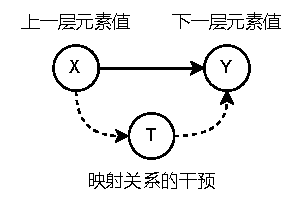
\includegraphics[width=0.45\textwidth]{pics/causal inference.pdf}
    \caption{卷积操作和自注意力操作的因果图}
    \label{fig:causal_inference}
\end{figure}

从因果推理的角度,可以对上述假设进行解释。图\ref{fig:causal_inference}展示了卷积操作和自注意力操作的因果图,其中$X$表示上一层的所有元素,$Y$表示下一层的所有元素,$T$表示某种映射关系的干预。对于自注意力操作来说,$X \to Y$表示自注意力操作,是一个全局映射,而$T$不存在,因此$X \to Y$之间不受任何干预。对于卷积操作来说,则是在$X \to Y$的基础上引入了某种映射关系的干预$T$,限制了$X$和$Y$之间的关系,使得全局关系变为局部关系。干预$T$可以形象地解释归纳偏置的作用,它使得空间上相近的元素之间更具有相关性,空间上不相近的元素之间几乎不具有相关性。

综上所述,CNN和ViT的差异主要在于操作的局部性质和全局性质,这一性质可能导致两种模型呈现出不同的现象:

\begin{itemize}
    \item CNN更适合建模局部关系,更关注局部细节特征,因为卷积操作是一种局部操作,可以有效地提取输入数据的局部特征,建模元素与附近元素之间的相关性。
    \item ViT更适合建模全局关系,更关注整体特征,因为自注意力操作是一种全局操作,可以对序列中任意两个元素之间的关系进行建模。
    \item 归纳偏置的假设可能导致两者在性能和泛化能力上的差异,这一假设可能会限制模型的性能,因为该假设不一定完全成立;该假设也可能会提高模型的泛化能力,因为在不同的任务下该假设可能是通用的。
\end{itemize}

在下面的章节中,我们将通过实验验证上述分析,比较CNN和ViT的特征表示,以及性能和泛化能力,探讨两者的差异和可能的内在原因。
